\documentclass{sig-alternate}
\usepackage{algorithm,algpseudocode}
\usepackage{url}

\begin{document}

\conferenceinfo{HPDC}{'12 Delft, The Netherlands}
% \CopyrightYear{2007} % Allows default copyright year (20XX) to be over-ridden
% - IF NEED BE. \crdata{0-12345-67-8/90/01}  % Allows default copyright data
% (0-89791-88-6/97/05) to be over-ridden - IF NEED BE.

\title{Cost- and Deadline-constrained Scheduling of Scientific Workflow Ensembles in IaaS Clouds}
% \subtitle{[Extended Abstract]}

\numberofauthors{2}
\author{
    \alignauthor Maciej Malawski and Jarek Nabrzyski\\
       \affaddr{University of Notre Dame}\\
       \affaddr{Center for Research Computing}\\
       \affaddr{111 Information Technology Center}\\
       \affaddr{Notre Dame, IN, USA}\\
       \email{\{mmalawsk,naber\}@nd.edu}
    \alignauthor Gideon Juve and Ewa Deelman\\
       \affaddr{USC Information Sciences Institute}\\
       \affaddr{4676 Admiralty Way}\\
       \affaddr{Marina del Rey, CA, USA}\\
       \email{\{gideon,deelman\}@isi.edu}
}

\maketitle
 
\begin{abstract}
Abstract goes here.
\end{abstract}

%\category{H.4}{Information Systems Applications}{Miscellaneous}
%\category{D.2.8}{Software Engineering}{Metrics}[complexity measures, performance measures]

%\terms{Theory}

\keywords{Scientific workflows, DAG scheduling, simulation}

\section{Introduction}

Scientific workflows, usually represented as directed acyclic graphs (DAG), are
the important class of applications that have been studied in the context of
resource management and scheduling on grid and utility computing systems.
However, large computational applications are not just individual workflows but
rather sets of inter-related workflows grouped in {\em ensembles}. All the
workflows in an ensemble typically have a similar structure, but they differ by
input data, number of tasks and individual tasks sizes. A good example of
scientific workflow ensemble comes from the CyberShake
application~\cite{Callaghan11}, which calculates seismic hazards for a given
geographical region such as California. In order to produce a hazard map, the
hazard curves need to be computed for a set of geographical sites, while each
site requires running a single complex scientific workflow. Workflows for each
site may differ not only by their parameters, but also by priority; e.g. some of
the points on the map correspond to urban areas or strategic locations such as
power plants, whereas others may be located in low populated regions. Another
examples of workflow ensembles come from astronomical applications, such as
Montage~\cite{Deelman08} or search for Earth-like planets from Kepler project
data~\cite{vockler11}, where multiple workflows are typically required to
process data covering different parts of the sky.
 
Infrastructure-as-a-service (Iaas) clouds offer capabilities of creating
(provisioning) computational resources on demand in a pay-per-use model and are regarded by
scientific community as a potentially attractive source of computing
resources~\cite{Ostermann10,Keahey09}. In contrast to clusters and grids which
typically offer best-effort resource provisioning capabilities, clouds give more
flexibility in terms of creating a controlled and managed computing environment
with the ability of adjusting resource capacity to the computing demands, often
called auto-scaling. Giving the users more control, however, clouds also require
developing new methods of task scheduling and resource provisioning. The
resource management decisions in cloud scenarios not only have to take into
account performance related metrics such as workflow makespan or resource
utilization, but also budget considerations, since the resources from public
(commercial) cloud providers are usually not free~\cite{Durkee10}.

In this paper, to get insight into these resource management challenges for
scietific workflow on clouds, we address a new important problem of maximizing
the number of completed workflows from an ensemble under both budget and
deadline constraints. The motivation is to answer the fundamental question of a
researcher: how much work can be completed in a limited budget and timeframe of
a research project. The goals of this paper are to discuss and assess possible
static and dynamic strategies for both task scheduling and resource
provisioning. Based on the knowledge of workflow scheduling algorithms we
analyze strategies for on-line scheduling of individual tasks as well as static
algorithms that rely on the information about the workflow structure (critical
paths and workflow levels) and estimates of task runtimes. In addition, we
analyze a hybrid workflow-aware dynamic scheduling algorithm, which uses the
workflow structure information to estimate which workflows should be rejected
from the ensemble due to the constraints. As methodology in the study of the
proposed algorithms we use simulation techniques. We have developed cloud workflow simulator based on
CloudSim~\cite{Calheiros11}, which models the infrastructure and the application. The
algorithms are subject to evaluation on a set of scientific workflow ensembles with a broad range of
budget and deadline parameters. 

The paper is organized as follows [\ldots]

\section{Related Work}
General policy and rule-based approaches to dynamic provisioning (e.g. Amazon
Auto Scaling\footnote{\url{http://aws.amazon.com/autoscaling}} and
RightScale\footnote{\url{http://www.rightscale.com}}).

Policy-based approaches for scientific workloads (e.g. \cite{Marshall2010, Kim2011}). Our approach is different in that we consider workflows, while policy based approaches typically consider bags of independent tasks or unpredictable batch workloads. This enables us to take advantage of scheduling heuristics that cannot be applied to independent tasks.

Deadline-constrained cost-minimization workflow scheduling. Our work is different from \cite{Yu2005, Abrishami2010} in that we consider ensembles of workflows in IaaS clouds, which allow one to provision resources on a per-hour billing model, rather than utility grids, which allow one to choose from a pool of existing resources with a per-job billing model. Our work is different from \cite{Mao2011} in that we consider ensembles of workflows rather than unpredictable workloads containing workflows. We also have budget constraints rather than cost minimization as a goal. In other words, we assume that there is more work to be done than the available budget, so some work must be rejected. Therefore cost is not something we optimize, but rather a constraint.

Budget-constrained workflow scheduling \cite{Sakellariou2007}.

Bi-criteria scheduling and multi-criteria scheduling. These approaches are similar to ours in that we have two scheduling criteria: cost and makespan. The challenge in multi-criteria scheduling is to derive an objective function that takes into account all of the criteria. These approaches typically use metaheuristics that run for a long time before producing good results.

\section{Problem Description}
\subsection{Resource Model}
Describe the Amazon EC2 resource model. Instances are requested on-demand. Instance pricing is per-hour. Multiple VM types are available, but for this paper we focus on a single VM type because we assume that there will typically be one VM type with the best price/performance ratio for the application.

\subsection{Application Model}
The target applications for this paper are scientific workflows that can be modeled as Directed Acyclic Graphs (DAGs).

We assume that we have runtime estimates for each task in the workflow.

Currently we do not consider data sizes, but rather assume that data is stored in a shared cloud storage system such as Amazon S3 and that data transfer times are included in task runtime estimates. Further, data transfer times are equal across the VMs.

An ensemble consists of several related workflows. Each workflow is given a priority.

The goal is to complete as many workflows as possible given a budget and a deadline.

\section{Algorithms}

\subsection{Static Provisioning Dynamic Scheduling\\
(SPDS) }
\label{sec:spds}
This is the simplest strategy based on static provisioning of resources and
on-line scheduling of workflow tasks. Given the budget $B$ and deadline $d$
together with the hourly price $p$ of a VM it is possible to compute the number
of VMs $N_{VM}$ to provision so that they consume the whole budget before the
deadline. 

\begin{equation}
\label{eq:static-plan}
N_{VM} = \lceil B / d / p \rceil
\end{equation}

Although simple, such provisioning plan has the advantage that it
minimizes the number of provisioning and deprovisioning requests.
Once the resources are provisioned, the tasks are scheduled to VMs using dynamic
priority-based Algorithm~\ref{alg:ds}. 

\begin{algorithm}
\caption{Priority-based scheduling}
\label{alg:ds}
\begin{algorithmic}[1]
\Procedure{schedule}{}
    \State $Q\gets set\ of\ released\ tasks$
    \State $P\gets empty\ priority\ queue$
    \While{$Q \neq \emptyset$}
    	\For{$task\ t\in Q$}
    		\State \Call{Insert}{$t,P$} 
    	\EndFor
    	\While{$FreeVMs \neq \emptyset \wedge P \neq \emptyset $}
    		\State $VM\gets$ \Call{SelectRandom}{$FreeVMs$}
    		\State $t\gets$ \Call{Pop}{$P$}
    		\State \Call{Submit}{$t,VM$}
    	\EndWhile
    	\State \Call{Wait}{$task\ finished$}
    	\State \Call{Update}{$Q$}
    \EndWhile
\EndProcedure
\end{algorithmic} 
\end{algorithm}

Initially all the
released tasks from all the workflows are submitted to the queue $Q$. Then, they
are inserted into priority queue $P$ based on the priority of workflows. If
there are free VMs available, the tasks from the priority queue are submitted to
the randomly choosen VMs. The process is repeated each time a task finishes.
Using the priority queue guarantees that tasks from lower priority workflows are
always submitted later than the higher priority ones and that the lower priority
tasks can occupy idle VMs. However, as there is no preemption, long-running
low-priority tasks may delay execution of high-priority tasks when such ones
become ready. Fig.~\ref{fig:spds-example} shows the example plan generated using
SPDS algorithm. It can be seen that tasks from lower priority workflows can fill
idle time of provisioned virtual machines.

\begin{figure}[htb] 
\centering
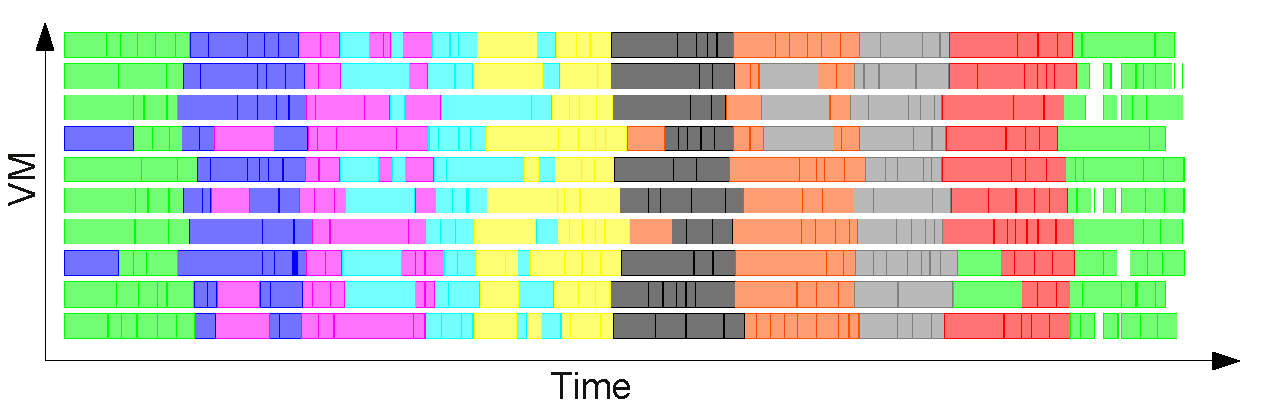
\includegraphics[width=1.0\columnwidth]{figures/spds-gantt}
 \caption{Example of schedule generated using SPDS algorithm: tasks are labelled
 by colors depending on the workflow. }
\label{fig:spds-example}
\end{figure}

\subsection{Dynamic Provisioning Dynamic Scheduling (DPDS)}

Static provisioning plan used in SPDS algorithm allows no changes to resource
pool at runtime. However, such plan may not be optimal when resource demand
changes during execution of workflows. In policy-based provisioning
(or auto-scaling) systems the metrics such as resource
utilization or queue length are typicaly used to estimate curret resource
demand. Our DPDS algorithm is based on resource utilization: the provisioner
module periodically computes utilization as the percentage of idle VMs. The
provisioner algorithm detects which VMs are finishing their hourly billing cycle
during the next provisioning period and decides whether they should continue
running, should be terminated or new VMs should be provisioned: see
Algorithm~\ref{alg:prov}.

\begin{algorithm}
\caption{Dynamic provisioner}
\label{alg:prov}
\begin{algorithmic}[1]
\Require $c$: consumed budget; $b$: total budget; $d$: deadline; $p$: price;
$t$: current time; $u_h$: upper utilization thershold; $u_l$: lower utilization
threshold.
\Procedure{provision}{}
    \State $V_C\gets set\ of\ VMs\ completing\ billing\ cycle$
    \State $n_T\gets\ 0$ \Comment{number of VMs to terminate} 
    \If{$ b - c < p * |V_C| \vee t > d $ }
    	\State $V_R\gets set\ of\ running\ VMs$
    	\State $n_T\gets |V_R| - \lfloor(b-c)/p\rfloor$ 
    	\State $V_T\gets select\ n_T VMs\ to\ terminate\ from\ V_C$
    	\State \Call{Terminate}{$V_T$}
    \Else 
    	\If{$u>u_h$}
    		\State \Call{Start}{$new\ VM$}
    	\EndIf
    	\If{$u<u_l$}
    		\State $V_F\gets free\ (idle)\ VMs$
    		\State $n_T\gets \lceil|V_F|/2\rceil$ 
    		\State \Call{Terminate}{$V_T$}
    	\EndIf 
    \EndIf
\EndProcedure
\end{algorithmic} 
\end{algorithm}

The number of instances to terminate $n_T$ computed in line 6 is the number that
would overrun the budget if not terminated. On the other hand $n_T$ computed in
line 15 prevents terminating all the instances too quickly, but makes sure that
if there is only one instance left it should be terminated. However, the
termination process is not immediate: to make sure that VMs that have been
already paid for are not terminated prematurely the {\em Terminate()} procedure
terminates only these instances that are close to the end of their billing
cycle. The remaining time threshold is calculated as a sum of provisioner
interval and estimated termination delay. This guarantees that no VMs can
overrun the assigned budget. To avoid uncontrolled increase of number of
instances, which may happen in the case of highly parallel workflows,
provisioner checks also the maximum scaling factor from the initial number of
provisioned VMs and prohibits starting new ones when this threshold is reached.


\subsection{Workflow-Aware DPDS (WA-DPDS)}

DPDS algorithm does not use any information about workflow structure: it deals
only with scheduling of individual released/ready tasks using their
workflow priorities. If there are no high priority tasks in the ready queue,
then lower priority tasks are submitted to idle resources. This may lead to the
deficiency in the following scenario: if a long-running task of low
priority is submitted to the idle machine and then several high
priority tasks are released to the ready queue, they become delayed by the
execution of the low priority task. This usually does not cause a problem when
the number of tasks and resources is high, but when the execution approaches the
budget and deadline constraint, we have observed that tasks of low-priority
workflows may prevent higher priority workflows from completion. This
observation leads to the improvemed algorithm which we call workflow-aware DPDS
(WA-DPDS).

WA-DPDS extends DPDS by introducing a workflow admission procedure, which is
invoked each time a task of a new workflow is at the head of priority queue,
i.e. just before it is submitted. The procedure estimates if there is enough
budget remaining to admit a new workflow: if not, all its tasks are rejected.
Algorithm~\ref{alg:wa-dpds} estimates the cost of admitting a new workflow and
compares it to the current cost (consumed budget) and remaining budget, taking
into account that started VMs have been already paid for. It adds a small safety
margin choosen to avoid overestimation of a budget.

\begin{algorithm}
\caption{Workflow admission algorithm for WA-DPDS}
\label{alg:wa-dpds}
\begin{algorithmic}[1]
\Require $w$: workflow; $b$: budget; $c$: current cost
\Procedure{Admit}{$w,b,c$}
    \State $r_n\gets b-c$ \Comment{Remaining budget for new VMs}
    \State $r_c\gets remaining\ cost\ on\ running\ VMs$
    \State $r_a\gets remaining\ cost\ of\ admitted\ workflows$
	\State $r_m\gets 0.1$ \Comment{Safety margin}
	\State $r_b\gets r_n+r_c-r_a-r_m$ \Comment{Budget remaining}
	\State $c_w\gets estimate\ cost(w)$
    \If{$c_w<r_b$}
    	\State \textbf{return} $TRUE$
    \Else
    	\State \textbf{return} $FALSE$
	\EndIf    	 
\EndProcedure
\end{algorithmic} 
\end{algorithm}


Admission procedure relies only on the total estimated resource consumption and
compares it to the budget remaining. We found that this estimation is useful not
only to prevent low-priority workflows from delaying ligh-priority ones, but
also in the case of ensembles consisting of workflows of non-uniform sizes, it
allows to reject big and costly workflows that would overrun the budget and
instead schedule some smaller ones to efficiently utilize idle resources. It
would be also possible to extend the admission procedure to check other
constraints, such as whether estimated critical path exceeds the deadline.



\subsection{Static Provisioning Static Scheduling (SPSS)}

We assume that the workflows are very wide such that the critical path of any given workflow is much less than the deadline.

The approach is to schedule each workflow in the ensemble in priority order, rejecting any workflows that cannot be completed by the deadline or that cause the cost of the plan to exceed the budget. Once the plan is complete, then the workflows are executed according to the plan.

\begin{algorithm}
\caption{Ensemble planning algorithm}
\label{alg:admit}
\begin{algorithmic}[1]
\Require $W$: workflow ensemble; $b$: budget; $d$: deadline
\Ensure Schedule as much of $W$ as possible given $b$ and $d$
\Procedure{PlanEnsemble}{$W,b,d$}
    \State $P\gets empty\ plan$
    \State $A\gets \emptyset$ \Comment{Set of admitted DAGs}
    \For{$w\ in\ W$}
        \State $P^\prime \gets$\ \Call{PlanDAG}{$w,P,d$}
        \If{$P^\prime\ is\ a\ valid\ plan$}
            \If{$Cost(P^\prime) \le b$}
                \State $P\gets\ P^\prime$ \Comment{Accept new plan}
                \State $A \gets A\ +\ w$ \Comment{Admit w}
            \EndIf
        \EndIf
    \EndFor
    \State \textbf{return} $P,A$
\EndProcedure
\end{algorithmic} 
\end{algorithm}


\begin{algorithm}
\caption{DAG planning algorithm}
\label{alg:plandag}
\begin{algorithmic}[1]
\Require $w$: DAG; $P$: current plan; $d$: deadline
\Ensure Create plan for $w$ that minimizes cost and meets deadline $d$
\Procedure{PlanDAG}{$w,P,d$}
    \State $P^\prime\gets$ copy of $P$
    \State \Call{DeadlineDistribution}{w,d}
    \For{$t\ in\ w\ sorted\ by\ Deadline(t)$}
        \State Choose resource r in $P^\prime$ that minimizes Cost(t)
        \If{$AFT(t,r) < Deadline(t)$}
            \State Schedule(t,r)
        \Else
            \State Provision a new resource r
            \State Schedule(t,r)
        \EndIf
    \EndFor
    \State \textbf{return} $P^\prime$
\EndProcedure
\end{algorithmic} 
\end{algorithm}


\begin{algorithm}
\caption{Deadline distribution algorithm}
\label{alg:deadlinedistribution}
\begin{algorithmic}[1]
\Require $w$: DAG; $d$: global deadline
\Ensure Assign sub-deadlines to each task in w
\Procedure{DeadlineDistribution}{$w,d$}
    \State $T \gets$ total number of tasks in $w$
    \State $R \gets$ total runtime of tasks in $w$
    \State $CP \gets$ length of critical path of $w$
    \State assign $Level(t)$ to each task $t$ in $w$
    \For{level $l\ \in w$}
        \State $Tasks(l) \gets$ number of tasks in $l$
        \State $Runtime(l) \gets$ runtime of tasks in $l$
        \State $r \gets \alpha * (Runtime(l)/R)$
        \State $t \gets (1-\alpha) * (Tasks(l)/T)$
        \State $FT(l) \gets (r + t) * (d - CP)$
    \EndFor
    \For{task $t \in w$}
        \State $LST(t) \gets \max(Deadline(p))\ for\ p \in Pred(t)$
        \State $Deadline(t) \gets LST(t) + RT(t) + FT(Level(t))$
    \EndFor
\EndProcedure
\end{algorithmic} 
\end{algorithm}

\begin{equation}
\label{eq:scaling}
FT(l) = \left[{\alpha}*\frac{T_l}{t}\right] + \left[{(1 - \alpha)}*\frac{R_l}{r} \right]
\end{equation}

\begin{figure}[htb] 
\centering
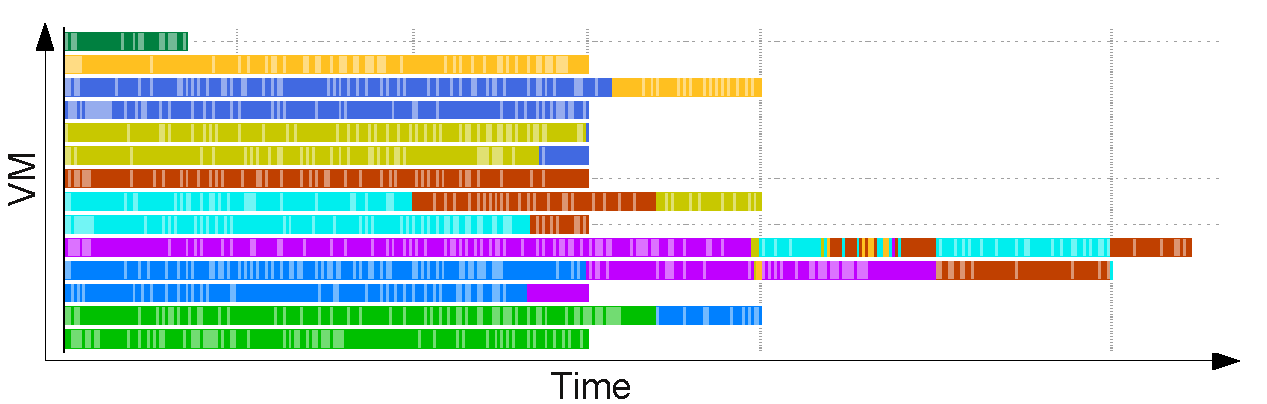
\includegraphics[width=1.0\columnwidth]{figures/spss-gantt}
 \caption{Example of schedule generated using SPSS algorithm: tasks are labelled
 by colors depending on the workflow. }
\label{fig:spss-example}
\end{figure}


\section{Performance Evaluation}

\subsection{Simulator}

\subsection{Scenarios}
\label{sec:scenarios}

We have prepared test scenarios to evaluate the proposed algorithms under
such a range of parameters that allows to observe the interesting properties of
algorithms for smaller and larger constraints. For a given ensemble we can
expect in general that the number of work done (in terms of workflows completed)
mainly depends on the budget constraint, which determines the number of
machine-hours that can be provisioned. The ideal but trivial case is then a
deadline long enough to allow running all the workflow tasks sequentially: this
eliminates all the overheads of parallel execution and leads to the highest
resource utilization. More interesting are the cases when the deadline is
shorter, since it forces provisioning of multiple VMs and thus increases
overheads due to parallel execution so the budget cannot be spent so
efficiently.

\begin{figure}[tb] 
\centering
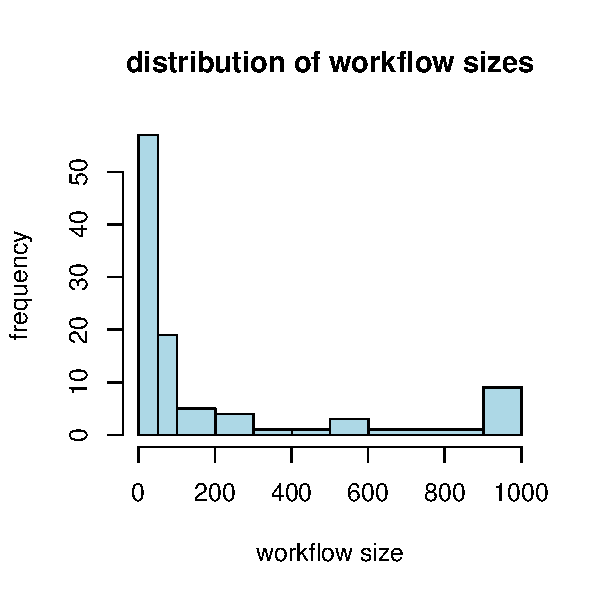
\includegraphics[width=0.6\columnwidth]{figures/ensemble-pareto}
\caption{Pareto-like distribution of workflow sizes in ensemble. Size is
measured in number of tasks.}
\label{fig:ensemble-distribution}
\end{figure}



We assumed that the interesting number of workflows in ensemble should be in the
order of between 10 and 100 workflows. This is motivated by several reasons:
first, such numbers are typical for the real applications, e.g. the number of geographical sites for
CyberShake workflow is in the order of 100. Second, the smaller ensembles
consisting of just a few workflows can be aggregated in a single workflow so
there is no need to treat them as ensembles. Similarly, when the number of
workflows is larger that 100 and each workflow has a large number of parallel
tasks, the problem of efficiently allocating them to the resources becomes much
easier and similar to the bag-of-tasks problem.


\begin{figure*}[t] 
\centering
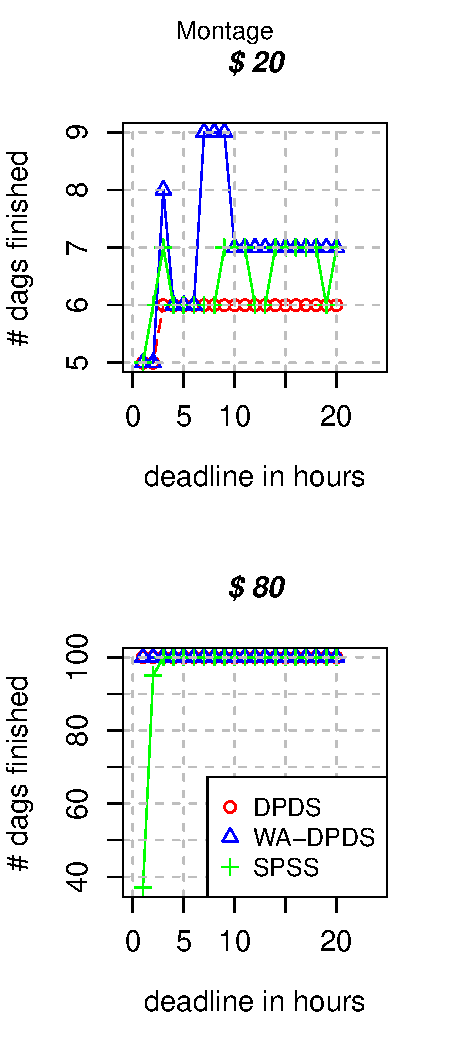
\includegraphics[width=0.19\textwidth]{figures/pareto-MONTAGE-n-1000-8-dagh1-20m0.pdf}
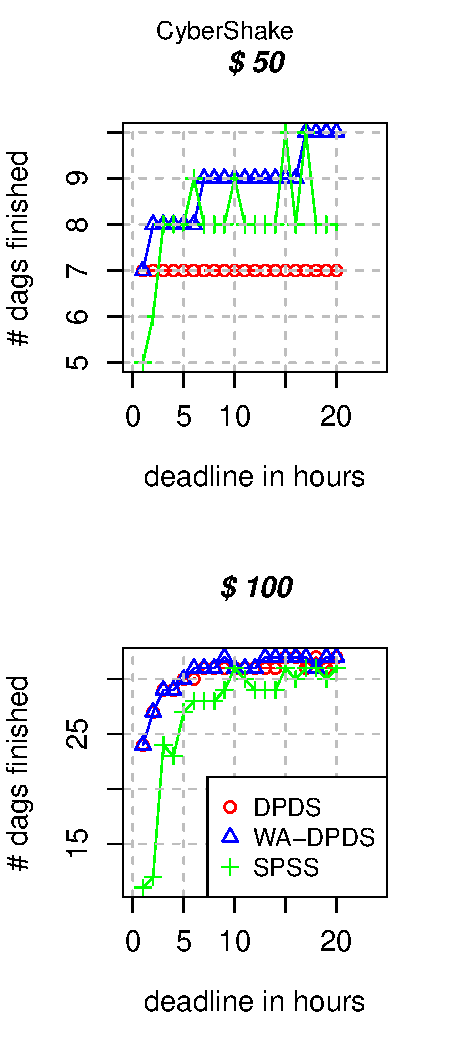
\includegraphics[width=0.19\textwidth]{figures/pareto-CYBERSHAKE-n-1000-8-dagh1-20m0.pdf}
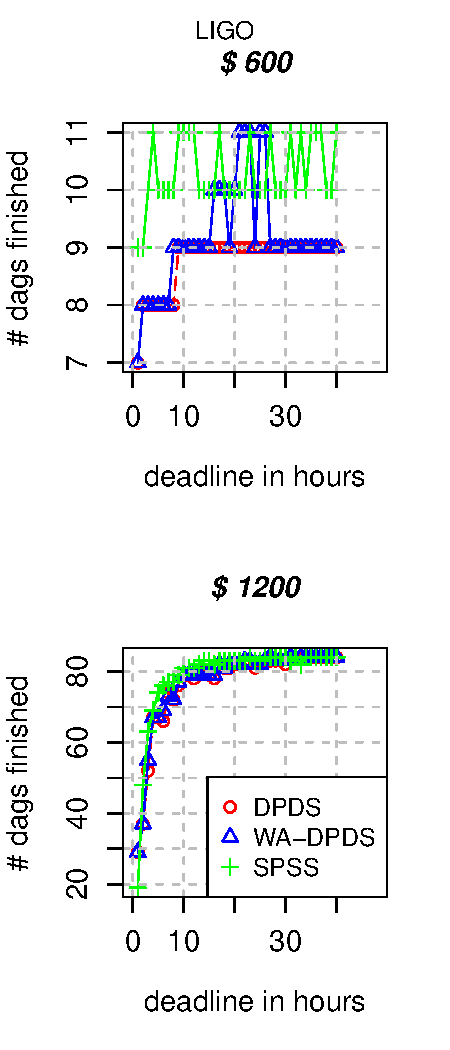
\includegraphics[width=0.19\textwidth]{figures/pareto-LIGO-n-1000-8-dagh1-40m0.pdf}
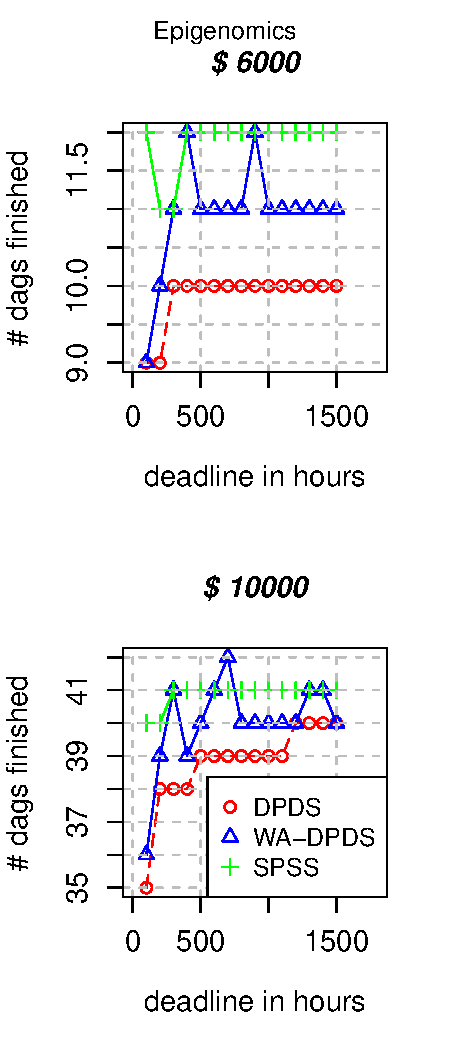
\includegraphics[width=0.19\textwidth]{figures/pareto-GENOME-n-1000-8-dagh100-1500m0.pdf}
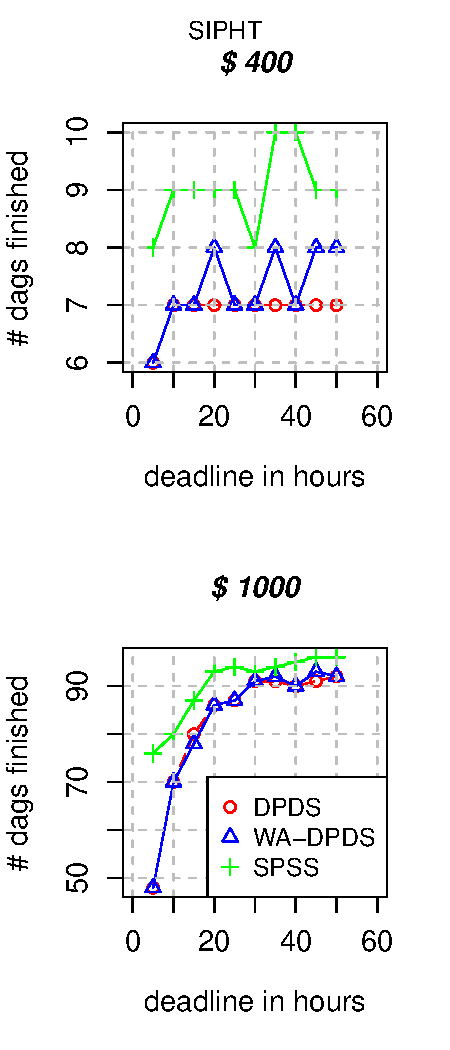
\includegraphics[width=0.19\textwidth]{figures/pareto-SIPHT-n-1000-8-dagh5-50m0.pdf}
\caption{Number of workflows completed for DPDS, AW-DPDS and SPSS
algorithms on ensembles of 100 Pareto-distributed workflows, {\em small budget}
(top) and {\em large budget} (bottom).}
\label{fig:number-complete-pareto}
\end{figure*}


%\begin{figure}[b!] 
%\centering
%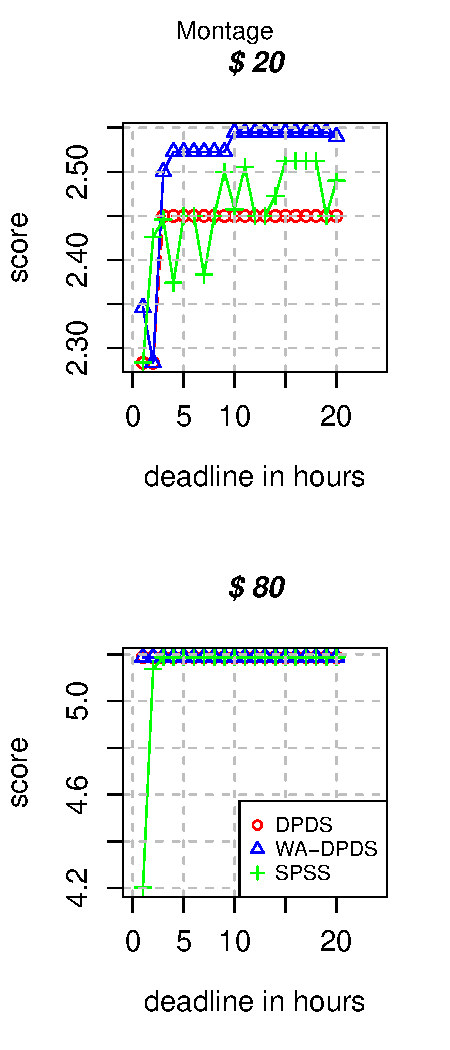
\includegraphics[width=0.19\textwidth]{figures/pareto-score-MONTAGE-n-1000-8-dagh1-20m0.pdf}
%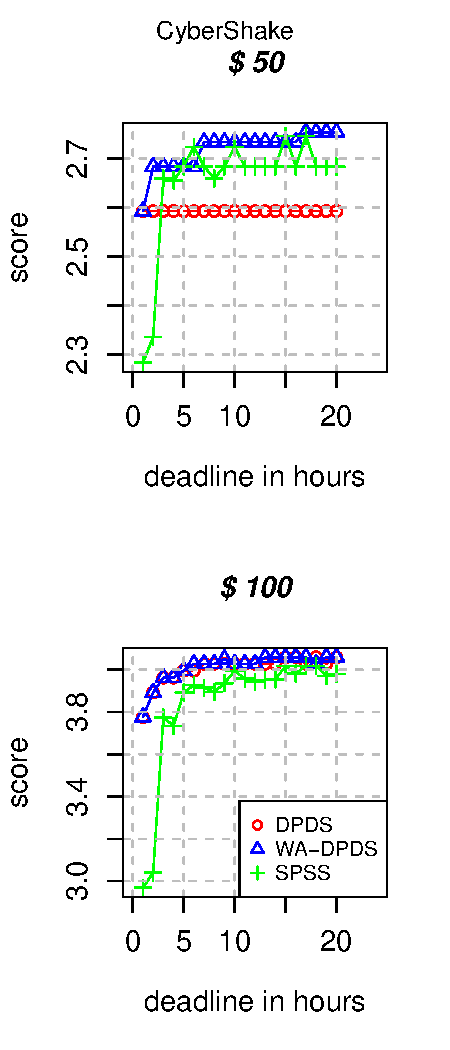
\includegraphics[width=0.19\textwidth]{figures/pareto-score-CYBERSHAKE-n-1000-8-dagh1-20m0.pdf}
%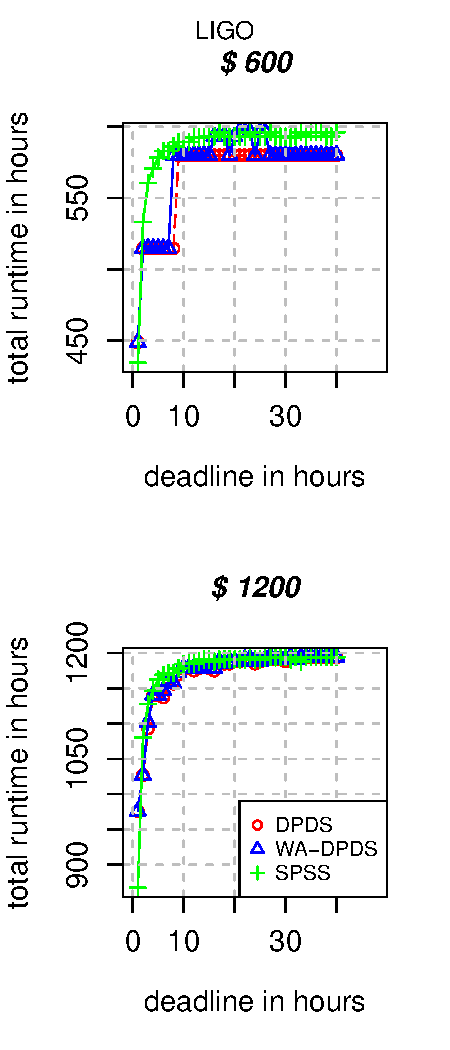
\includegraphics[width=0.19\textwidth]{figures/pareto-score-LIGO-n-1000-8-dagh1-40m0.pdf}
%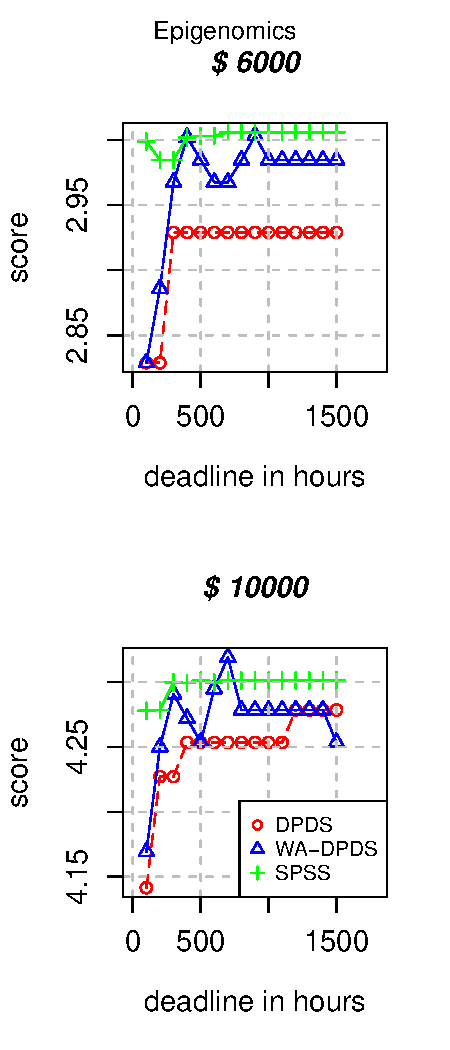
\includegraphics[width=0.19\textwidth]{figures/pareto-score-GENOME-n-1000-8-dagh100-1500m0.pdf}
%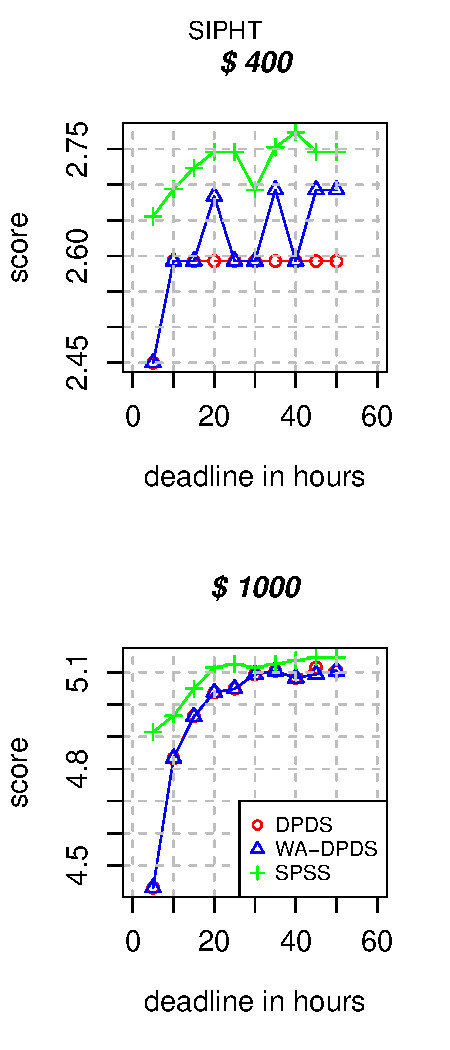
\includegraphics[width=0.19\textwidth]{figures/pareto-score-SIPHT-n-1000-8-dagh5-50m0.pdf}
%\caption{Comparison of algorithms based on score, which  is computed as
%$\sum(1/(p+1))$ where priorities of subsequent workflows are $p=0,1,2,\ldots$
%(0 means highest priority).}
%\label{fig:score}
%\end{figure}




In order to evaluate the algorithms on a standard ser of workflows, we used
ensembles constructed from the DAGs available\footnote{\url{https://confluence.pegasus.isi.edu/display/pegasus/WorkflowGenerator}}
in the workflow generator gallery~\cite{Bharathi08}. The gallery contains
workflows of five applications from Pegasus and from Indiana
University~\cite{Ramakrishnan08}. We constructed ensembles of 100 DAGs by sampling the
workflows of different sizes based on a given distribution. By the size of the
workflow means the number of jobs. Two distributions are considered:
\begin{itemize}
  \item ensemble of workflows of equal size (constant)
  \item Pareto-like distribution.
\end{itemize}

Pareto-like distribution gives a small number of workflows with large size and a
large number of workflows with small size, as seen in
Fig.~\ref{fig:ensemble-distribution}. The number of largest
workflows (of size $\geq$ 900) is slightly increased to represent the
``long-tail'', i.e. that there is a non-insignificant number of large workflows
in the ensemble. The workflows are sorted according to their size and the largest workflows are
given the highest priority. 




\begin{figure*}[t]  
\centering
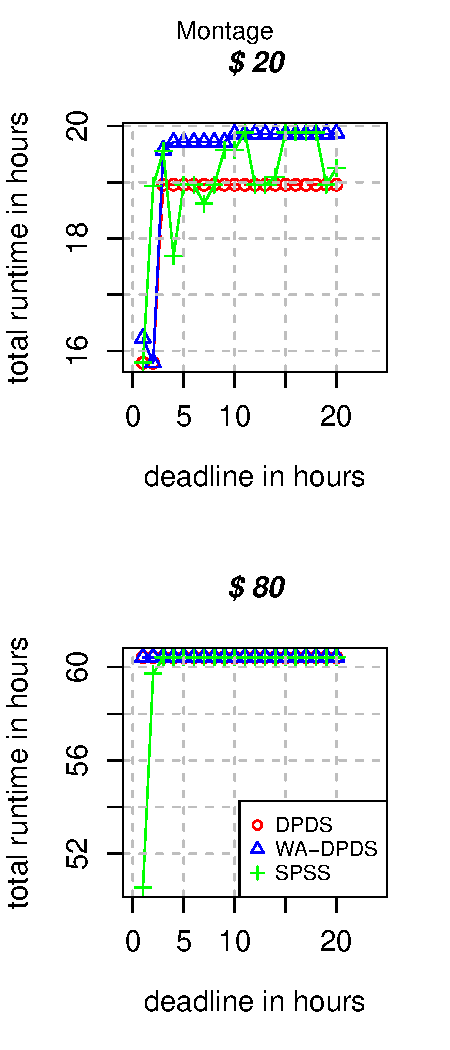
\includegraphics[width=0.19\textwidth]{figures/pareto-size-MONTAGE-n-1000-8-dagh1-20m0.pdf}
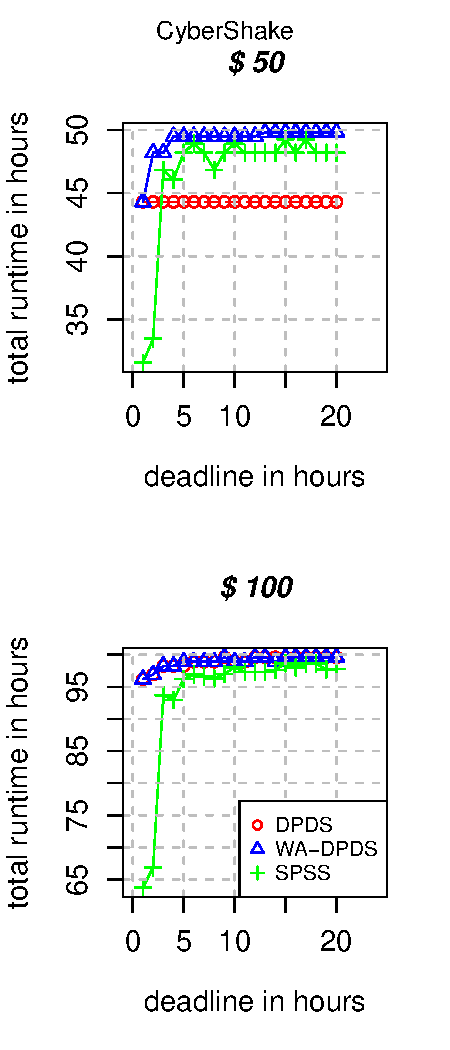
\includegraphics[width=0.19\textwidth]{figures/pareto-size-CYBERSHAKE-n-1000-8-dagh1-20m0.pdf}
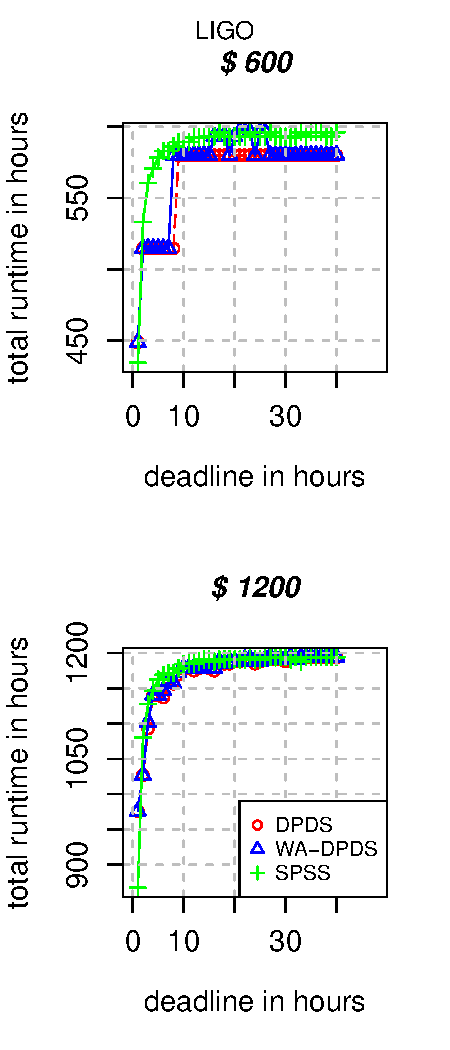
\includegraphics[width=0.19\textwidth]{figures/pareto-size-LIGO-n-1000-8-dagh1-40m0.pdf}
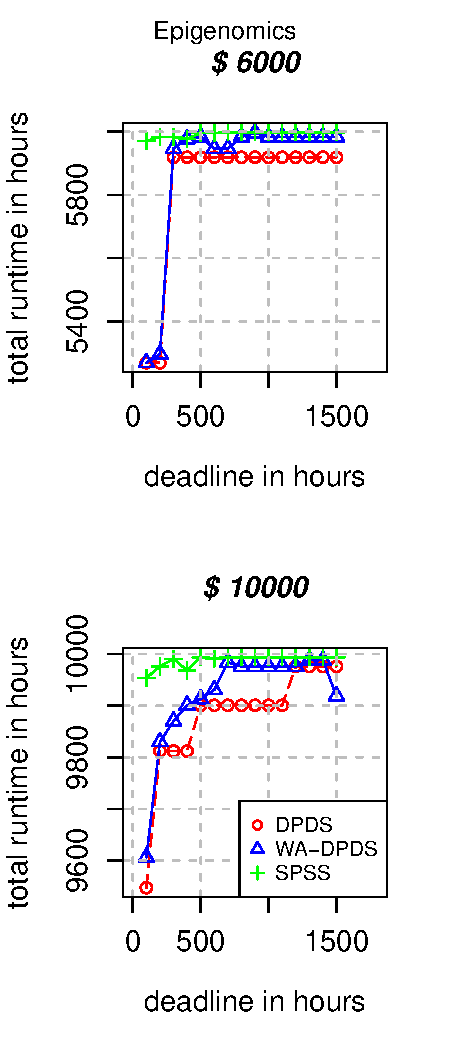
\includegraphics[width=0.19\textwidth]{figures/pareto-size-GENOME-n-1000-8-dagh100-1500m0.pdf}
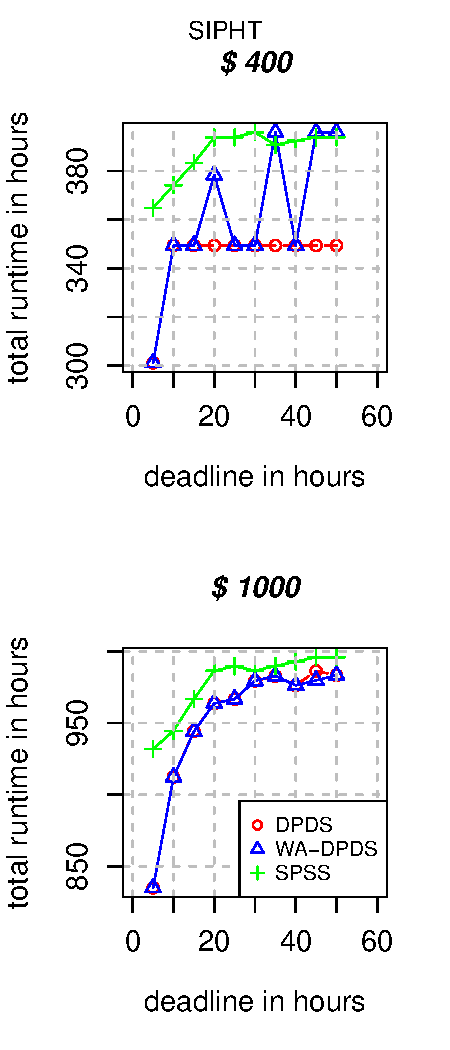
\includegraphics[width=0.19\textwidth]{figures/pareto-size-SIPHT-n-1000-8-dagh5-50m0.pdf}
\caption{ Total work completed expressed as the sum of runtimes (in hours) of
tasks of completed workflows. Data computed for DPDS, AW-DPDS and SPSS
algorithms on ensembles of 100 Pareto-distributed workflows}
\label{fig:total-time}
\end{figure*}


In the tests we we assumed that all the VMs are homogeneous and have the
processing speed of 1000 MIPS (million instructions per second), the price for
one VM-hour is \$1 and that the sizes of tasks in the workflow gallery are given
in seconds measured on 1000 MIPS machines. In this study we do not take into
account the heterogeneity of the infrastructure since we assume that it is
always possible to select a VM type that has the best price to performance ratio
for a given application.

For each application type, we selected such ranges of constraints (deadline,
budget) that it is possible to observe the possibly broad result space: from the
tight constraints, when only a small number of workflows can finish to the
liberal constraints when all or almost all the workflows can finish. These
parameters vary among the applications. Montage and CyberShake benchmarks
workflows required the budget in \$20 -- \$150 range and deadlines from 1 to
20 hours to complete the ensemble. LIGO and SIPHT workflows have more long
tasks, so they require budgets up to \$1,500 and deadlines extended to 40
hours. Epigenomics workflow is even more costly and needs approximately \$12,000
and 1500 hours to complete the full ensemble.

We show the results of three algorithms (TODO: ADD MORE): DPDS, WA-DPDS and
SPSS. These tests were run with maximum autoscaling factor set to 1.0 for
DPDS and WA-DPDS. After experimenting with DPDS and WA-DPDS we found that due to
high parallelism of workflows the resource utilization remains high most of the time, 
which leads to rapid provisioning of new resources at the beginning of ensemble
execution. This in turn results in less efficient total utilization due to high
level of parallelism. Setting the scaling limit to 1.0, ensures that the shape
of resource provisioning plan is closest to a rectangle (see
Fig.~\ref{fig:spds-example}) and the VM termination procedure
(Algorithm~\ref{alg:prov}) allows maximum utilization of VMs before shutdown.




\subsection{Metrics}




There are multiple ways to evaluate the algorithms and also different metrics
are relevant to the application users that are needed to take the planning
decisions. The set of metrics for each ensemble run we prepared includes:
\begin{itemize}
  \item number of workflows completed $N_c$,
  \item user preference score (utility function) $s$,
  \item total amount of computing time completed $T_C$,
  \item effective cost of computing per hour $C_{eff}$, which includes
  overheads.
\end{itemize}


The number of workflows completed is a simplest metric and allows distinguishing
which algorithm performs better. However, as the workflows have
different priorities and sizes, a less efficient algorithm may schedule smaller
low-priority workflows first, thus increasing the total number of workflows
complete. It may also happen that too conservative admission algoritm may reject
overestimate the costs of some large workflows, thus rejest some high-priority
ones which actually could fit into the schedule. Therefore we defined a user
preference score as:

%\begin{equation}
%\label{eq:score}
%s = \sum_{DAGs\ completed}(1/(p+1))
%\end{equation}


\begin{equation}
\label{eq:score}
s = \sum_{DAGs\ completed}2^{-p}
\end{equation}


where priorities of subsequent workflows in the ensemble are $p=0,1,2,\ldots$ (0
means highest priority). This exponential scoring function gives a strong weight
to the top priority workflows, since it has a property that a score for
completing a single workflow with priority $p$ is higher that the score for
completing all lower priority ones: 
\begin{equation}
\label{eq:score-property}
2^{-p} > \sum_{i=p+1,\ldots}2^{-i}
\end{equation}

Another metric is the total actual computing time completed and it is calculated
as the sum of all the runtimes of all the tasks of completed workflows. As in
our study we assumed that the resource cost pre hour is equal to \$1, the total
computing time can be easily compared to the allocated budget $b$. Their ratio
$u = (T_C * \$1)/b$ is the resource utilization and its inverse is the effective
resource cost: $C_{eff} = b/T_C$ in dollars per hour.

\subsection{Discussion of Results}




We run the simulations for the constraint values ranging between the
estimated limits as indicated in Section~\ref{sec:scenarios}, resulting in
ca. 50-150 (budget, deadline) points for each application. The runs were
repeated for Pareto-distributed and costant workflow sizes. From this result
space we selected the most interesting plots which give the good overview  of
the observed algorithm behavior.





\begin{figure*}[htb] 
\centering
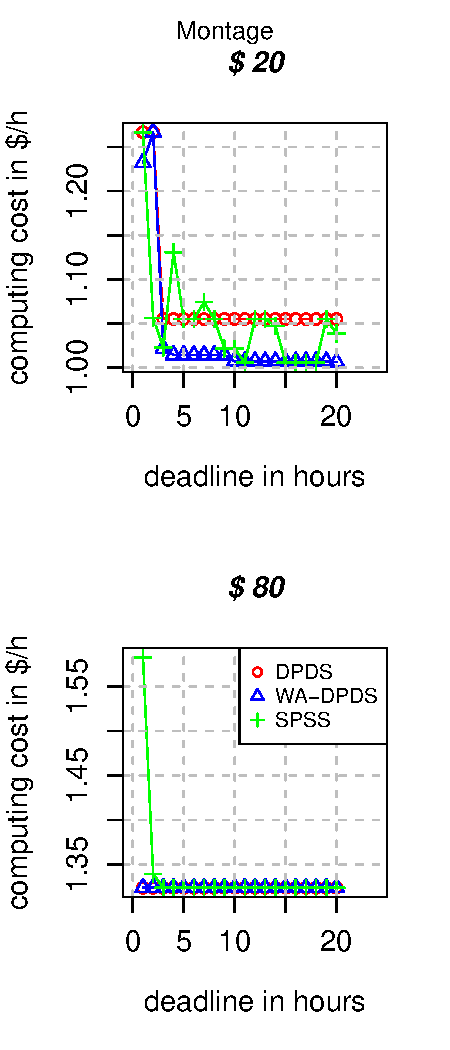
\includegraphics[width=0.19\textwidth]{figures/pareto-cost-MONTAGE-n-1000-8-dagh1-20m0.pdf}
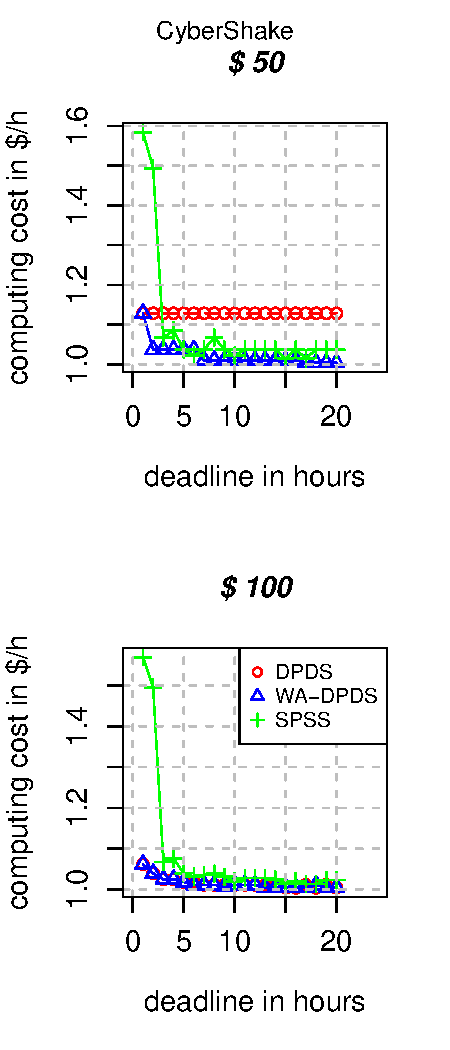
\includegraphics[width=0.19\textwidth]{figures/pareto-cost-CYBERSHAKE-n-1000-8-dagh1-20m0.pdf}
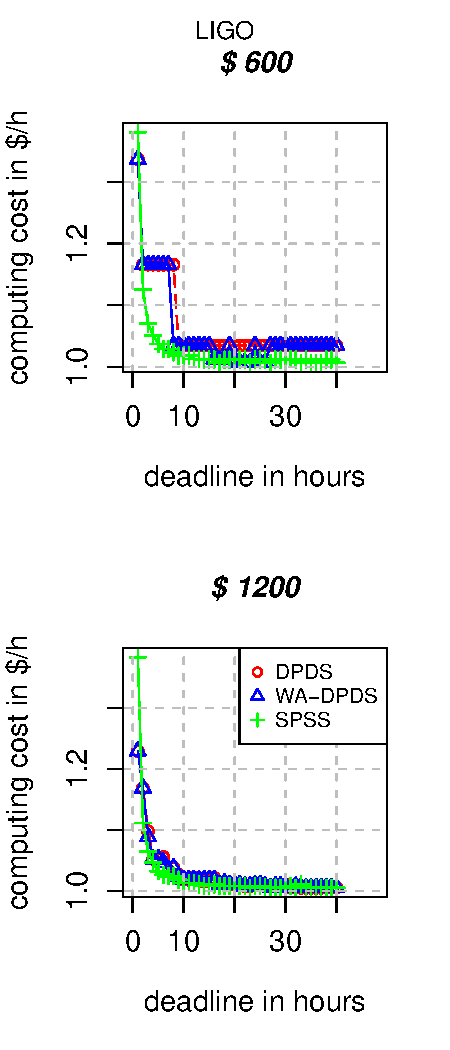
\includegraphics[width=0.19\textwidth]{figures/pareto-cost-LIGO-n-1000-8-dagh1-40m0.pdf}
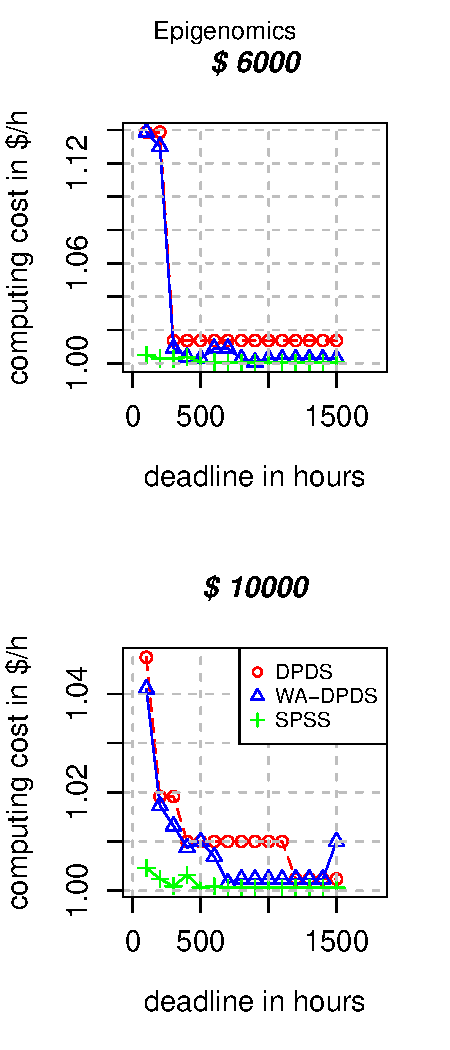
\includegraphics[width=0.19\textwidth]{figures/pareto-cost-GENOME-n-1000-8-dagh100-1500m0.pdf}
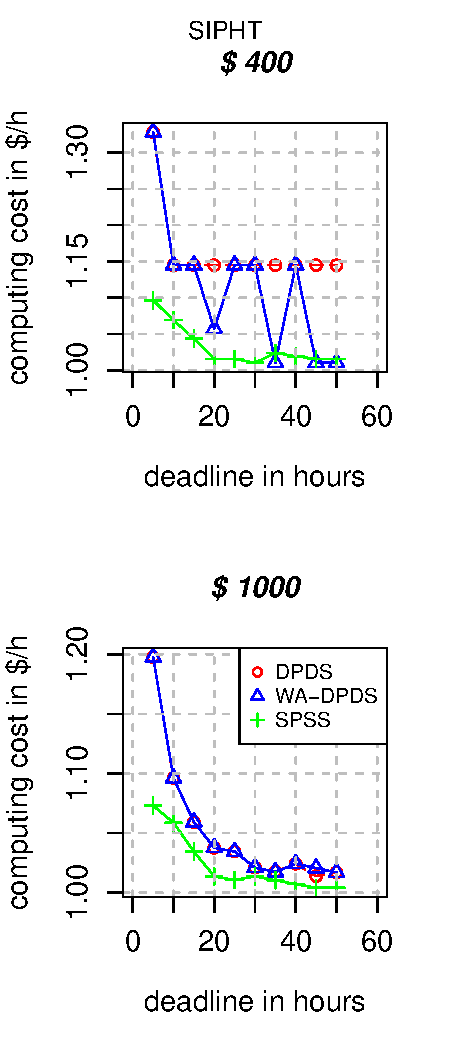
\includegraphics[width=0.19\textwidth]{figures/pareto-cost-SIPHT-n-1000-8-dagh5-50m0.pdf}
\caption{Effective computing cost in \$ per hour calculated by dividing sum of
task runtimes by the total budget. Higher cost results from lower resource utilization. Data based on DPDS, AW-DPDS and SPSS algorithms for ensembles of 100
Pareto-distributed workflows.}
\label{fig:cost}
\end{figure*}



Fig.~\ref{fig:number-complete-pareto} shows the number of the workflows
completed for two budget values per each application ensemble. The budget values
selected correspond to two opposite cases: {\em small budget} (top) and {\em
large budget} (bottom). The first one allows completing only a small number of
workflows from the ensemble, while the latter one suffices to finish almost all
the workflows. It can be seen that the static planning algorithm (SPSS) performs
better for tighter constraints: when the budget is low to admit only a small
number of workflows, the static procedure is able to more efficiently pack these
workflow tasks onto the resources. This can be clearly seen for the LIGO,
Epigenomics and SIPHT ensembles for small budgets and also for the same
ensembles with large budgets but short deadlines. The exception are Montage and
CyberShake ensembles, which consist of many fine-grained tasks that can be
executed in parallel. For these cases, as well for the other ensembles with
large budgets, the simple dynamic scheduling techniques perform equally well or
better. The reason for that behavior is that the large number of tasks
guarantees that resources are almost never idle, while the provisioner algorithm
makes sure that the VM instances are most efficiently utilized before shutdown.
We can also observe that the workflow-aware dynamic algorithm (WA-DPDS) performs
better than the workflow-unaware version. This means that for the tested
workflows the simple admission procedure based on estimation of workflow cost
does not degrade the solution, but rather in many cases it allows rejecting
larger workflows that would lead to budget overrun. Thus it can save the space
for smaller workflows that can complete.





%Fig.~\ref{fig:score} shows the score $s$ as defined in Eq.~\ref{eq:score}
%computed for two sample applications. Comparing
%Fig.~\ref{fig:number-complete-pareto} to Fig.~\ref{fig:score} we can see that
%the latter one gives more flattened shape: this means that e.g. the improvement
%of the solution by one workflow may mean adding a one low-priority workflow.
%Nevertheless we can see that the curves on both figures have a very similar
%shape, which mens that our algorithms obey the priority rules and do not try to
%admit lower-priority workflows at the cost of the more important ones.

\begin{figure}[htb] 
\centering
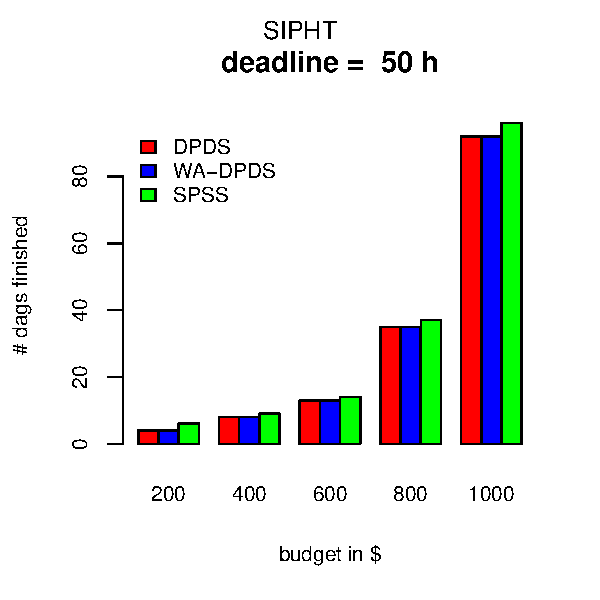
\includegraphics[width=0.6\columnwidth]{figures/pareto-budget-SIPHT-n-1000-8-dagh5-50h10m0.pdf}
\caption{Comparison of number of workflows completed for a given deadline,
plotted versus different budget amounts.}
\label{fig:budgets}
\end{figure}



\begin{table}[tb]
\centering

(a) Number of workflows completed $N_c$:
\medskip
\begin{tabular}{r|cccccc}
 & M & C & L & E & S & TOTAL\tabularnewline
\hline
DPDS      &   57  & 45 &  18 &  14  &  0 & 134\tabularnewline
WA-DPDS   &    96 &  87  & 48  & 34  &  0 & 265\tabularnewline
SPSS     &    29  & 42  & 192  & 74  & 50 & 387\tabularnewline
\end{tabular}
\medskip

(b) Total amount of computing time completed $T_C$:
\medskip
\begin{tabular}{r|cccccc}
 & M & C & L & E & S & TOTAL\tabularnewline
\hline
DPDS      &   58  & 45 &  19 &  14  &  0 & 136\tabularnewline
WA-DPDS   &    90  & 96  & 57  & 27 &   8 & 278\tabularnewline
SPSS     &    31 &  18 &  170  & 75 &  42 & 336\tabularnewline
\end{tabular}
\medskip

(c) Exponential score $s$:
\medskip
\begin{tabular}{r|cccccc}
 & M & C & L & E & S & TOTAL\tabularnewline
\hline
DPDS      &   58 &  45 &  46 &  15  &  9 & 173\tabularnewline
WA-DPDS   &    90 &  96  & 84  & 29 &  17 & 316\tabularnewline
SPSS     &    48 &  27 & 173 &  75 &  42 & 365\tabularnewline
\end{tabular}
\medskip


M -- Montage; C -- CyberShake; L -- LIGO; E -- Epigenomics; S --SIPHT

\label{tab:num-dags-pareto}
\caption{Number of times each algorithm achieved the highest score for each
application (over all budgets and deadlines). Data based on total 525 runs on Pareto-distributed ensembles.}
\end{table}


Fig.~\ref{fig:total-time} presents the same results using the total computing
time metric $T_C$. These plots confirm our previous observations about the
algorithms performance, but they also allow to observe a more general property.
For a given budget, when the deadline is tightened the number of work done
steeply decreases. Assiging a shorter deadline means that more VMs need to be
provisioned to complete the work, but this leads to higher parallelism and thus
to the lower parallel efficiency. E.g. running 2 VMs for 10 hours will be more
efficient than running 10 VMs for 2 hours. Therefore, if deadline permits and
costs are important, parallelism should be avoided when possible.

These observations are further confirmed when examining the efffective resource
cost, as shown in Fig.~\ref{fig:cost}. It can be seen that lower resource
utilization and lower parallel efficiency for short deadlines lead to
substantial increase of actual costs of computing. This increase reaches
$\sim$20\%, which means that if we need to run e.g. a SIPHT workflow ensemble
with a short deadline, $\sim$\$200 out of \$1000 is spent on idle resources.

Another general conclusion can be drawn from Fig.~\ref{fig:cost}: despite some
random fluctuations resulting mostly from the finite result space, all the
curves for all the applications and budgets have a similar shape. This shape
represents a trade-off curve between two conflicting objectives: time and cost.
We can see that the selection of deadline and cost can be formulated as
multi-criteria optimization problem and the curves presented in
Fig.~\ref{fig:cost} are approximations of the Pareto front (or Pareto set) of
solutions to this problem. In our case the solutions were achieved by maximizing
the number of work done, which direcly results in minimization of effective cost parameter for a given
deadline. Therefore, the obtained results can be used to assist the decison in
resource allocation planning, when both cost and time criteria are given not as
constraints but as objectives.


% \begin{figure*}[htb] \centering
% 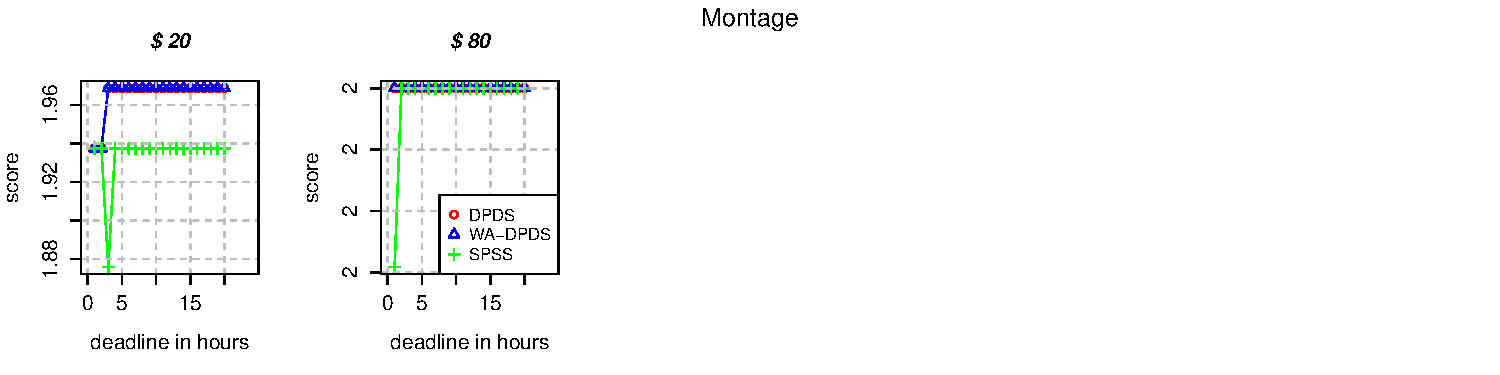
\includegraphics[width=0.19\textwidth]{figures/score2-MONTAGE-n-1000-8-dagh1-20m0.pdf}
% 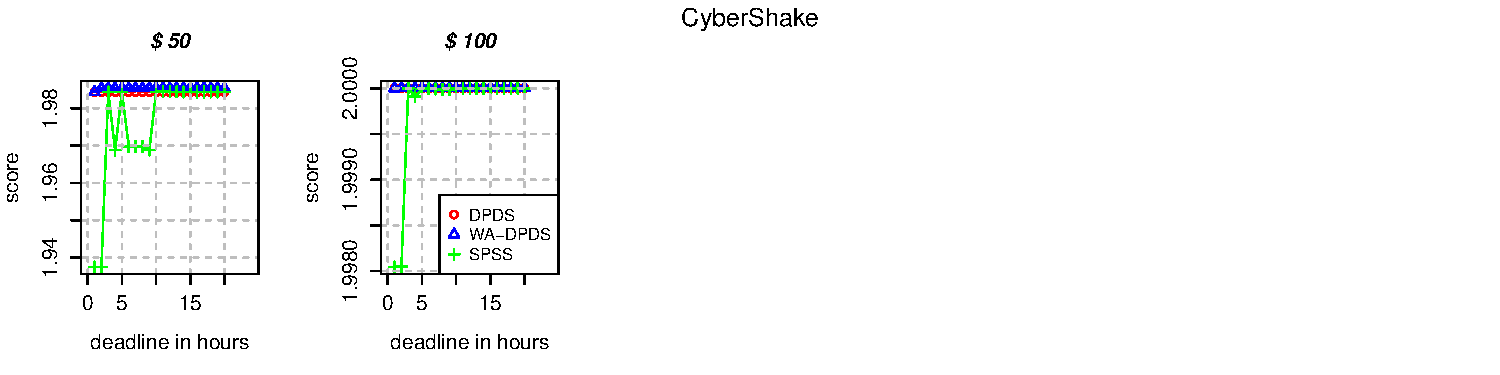
\includegraphics[width=0.19\textwidth]{figures/score2-CYBERSHAKE-n-1000-8-dagh1-20m0.pdf}
% 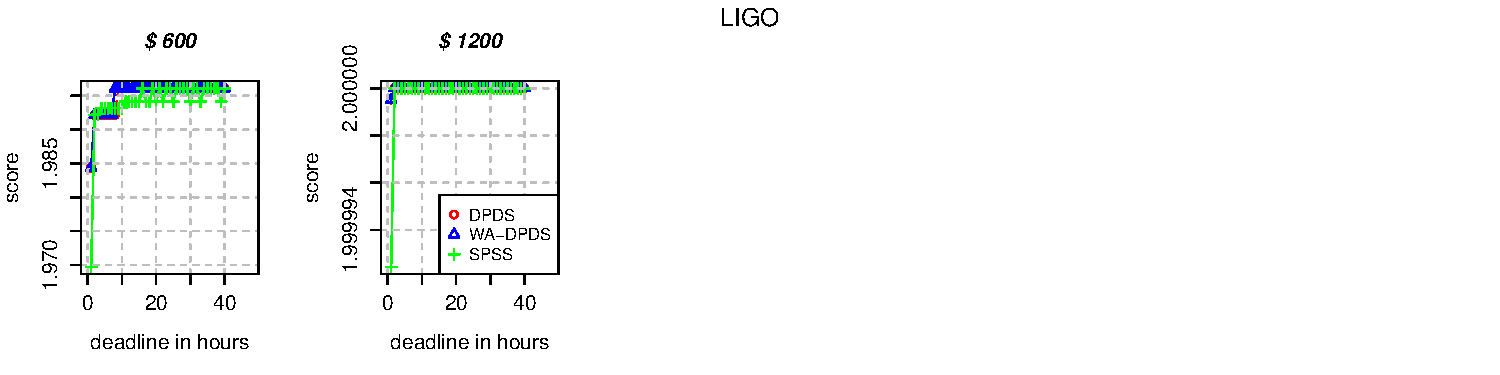
\includegraphics[width=0.19\textwidth]{figures/score2-LIGO-n-1000-8-dagh1-40m0.pdf}
% 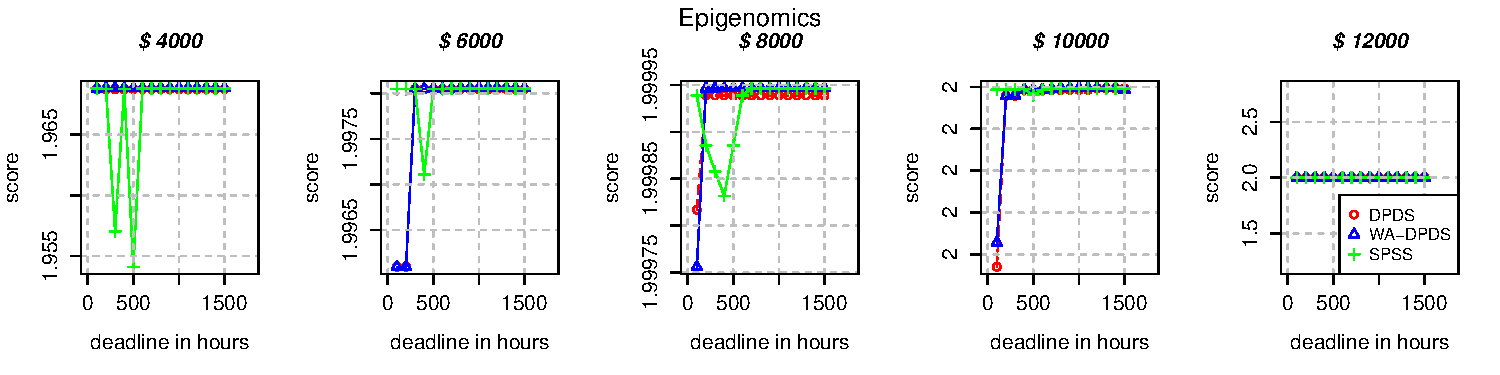
\includegraphics[width=0.19\textwidth]{figures/score2-GENOME-n-1000-8-dagh100-1500m0.pdf}
% 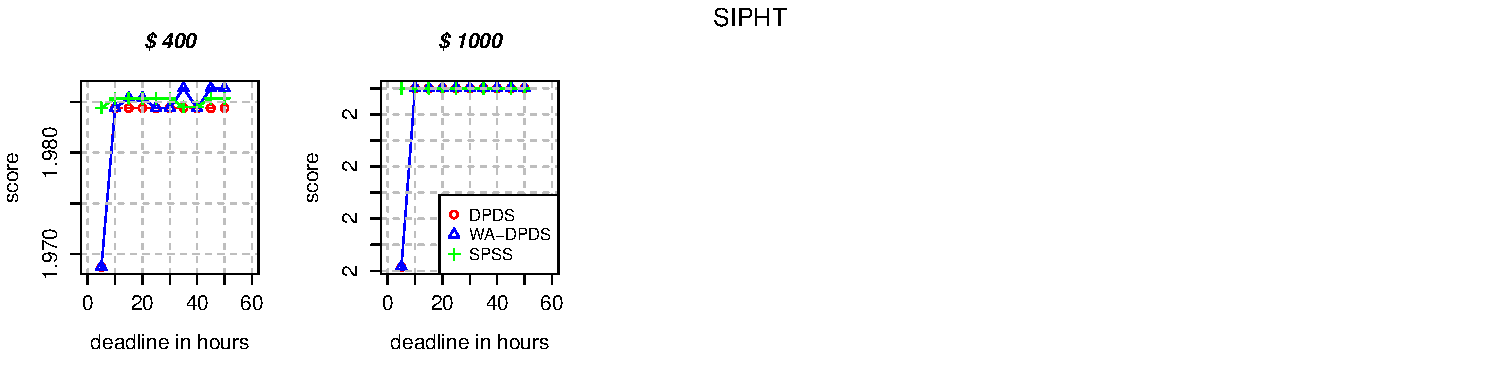
\includegraphics[width=0.19\textwidth]{figures/score2-SIPHT-n-1000-8-dagh5-50m0.pdf}
% \caption{Comparison of DPDS, AW-DPDS and SPSS algorithms for ensembles of 100
% Pareto-distributed workflows. Score is computed as $\sum(2^(-p))$ where
% priorities of subsequent workflows are $p=0,1,2,\ldots$ (0 means highest
% priority).} \label{fig:} \end{figure*}
       
               
In order to compare efficiency of algorithms, we counted the number of times
each algorithm achieved the best results for all tested applications, deadlines
and budgets. If two or more algorithms achieve the same highest results, all are
counted as highest. Table~\ref{tab:num-dags-pareto} shows these summary values.
These results depend on the metric: number of workflows completed does not count
the priorities or sizes of workflows, which means that it happens more often
that all the algorithms achieve the same (best) result. However, it does not
mean that all algorithms complete the same workflows: that is why values
in the tables (a), (b) and (c) are different. it can be observed that based on
the sampled problem space the workflow-aware algorithms achieve highest score
in $\sim$2--3 times more cases than the simple DPDS which does not take into
account workflow structure or size. In average, SPSS performs better in
$\sim$20--50\% more times than WA-DPDS. We have to note, that the sampled
paramter space included the Montage and CyberShake workflows consisting of many
small tasks, for which cases SPSS does not perform equally well. 
               
               
Fig.~\ref{fig:budgets} whows the same data for SIPHT ensemble from another
perspective. It helps answer the question: given a deadline, how many workflows
can be finished when we increse the budget. In Fig.~\ref{fig:budgets} the growth
is super-linear, what results from the distribution of workflow sizes in the
ensemble (see Fig.~\ref{fig:ensemble-distribution}). For ensemble of equal size
workflows (see Fig. TODO: ADD FIGURE FROM CONSTANT DISTRIBUTION) the growth is
nearly linear. It can be also observed that staitc algorithms give better
results for smaller budgets, while dynamic algorithms for larger ones.




\section{Conclusion and Future Work}

In this paper we addressed a new interesting and important problem of scheduling
and resource provisioning for scientific workflow ensembles on IaaS cloud
infrastructures. The problem is different from previous work on grid or utility
grid scheduling that cloud infrastructure gives more control over the resources,
so the resource provisioning plan can be adjusted to the application
requirements. Therefore the problem space becomes larger: it requires not
only to select the best scheduling of tasks to available resources, but also
select the best shape of resource provisioning plan. The formulation of a
problem as maximization of the number of prioritized workflows completed from
the ensemble requires also to take the decisions on admitting or rejecting workflows
based on their estimated resource demands. We believe that such formulation of
the bi-constrained problem is highly relevant since such
constraints are typically imposed on many real-world projects.

We have analyzed both static and dynamic scheduling approaches and
developed the SPDS, DPDS, WA-DPDS and SPSS algorithms realizing these
strategies. The algorithms were evaluated on ensembles of benchmark
workflows which represent typical real scientific applications. For the
purpose of evaluation we have developed a simulator that models the cloud
infrastructure and the tightly-coupled scheduler and provisioner modules of
workflow engine. The results of simulation studies indicate that the two algorithms (WA-DPDS and
SPSD) that take into account the information about the workflow structure and
estimation of task runtimes yield better results than the simple on-line
priority-based scheduling strategy with static (constant) resource provisioning
plan. 

During our work, several interesting lessons were learned about the workflow
ensembles on cloud infrastructures. One result is that the simple strategy of
SPDS performs relatively well in terms of number of workflows completed and the
high resource utilization it can achieve. However, this method does not allow to
give any advance prediction about the result, so to see its performance the
whole ensemble needs to be simulated. On the other hand, the method may be
the only choice in the case no estimates about the task runtimes are available
in advance. It can be seen that the workflow-aware and static algorithms are
able to find better quality solutions in terms of the defined metrics: this the
result mainly of the admission algorithm implemented, which allow rejecting too
large workflows and thus saving resources for completing the less costly ones.

Another general observation is that although clouds provide such capabilities as
dynamic adding and removing of resources at runtime and high parallelization due
to ilusion of unlimited resources, it turns out that is recommended to avoid
using these capabilities when possible, in order to achieve high resource
utilization and cost effectiveness. This observation comes from the fact that
starting and stopping more VMs incurres a cost which can be amortized by running
each started VM as long as possible before shutdown. This effect was confirmed
in the case of SPSS algorithm for Montage and CyberShake workflows with small
budgets. Similarly, high degree of parallelization (large number of nodes) leads
also to less efficient resource utilization and in the case of clouds the drop
in parallel efficiency means also the increase of cost. This result, clearly
visible in Fig~\ref{fig:cost}, leads to multi-criteria decision problems and
related trade-offs. E.g. our simulation results can be used as hints to answer
the question how much time and money is required to actually complete all the
workflows from the given ansemble.

Another lesson learned from our studies is related to the shapes and granularity
of the tasks of workflows in the ensembles. The benchmarks workflows that we
tested have relatively large number of tasks (50--1000). Montage and CyberShake
workflows have fine-grained tasks of short execution times, in the order of
seconds and minutes. LIGO, Epigenomics and SIPHT have longer tasks: from minutes to hours.
Therefore the dynamic algorithms achieved better results on the fine grained
workflows, since the simple random-based allocation strategy leads to good
load-balancing and high resource utilization. On the other hand, when tasks are
longer, it becomes more beneficial to apply a static planning strategy of SPSS.

Our current study reveals multiple paths for future work. One interesting
question would be to answer how the static and dynamic algorithms perform in the
cases of increased uncertainities and failures, that have important influence
on overall system performance~\cite{Sakellariou2010,Dongarra2007}. Second
important goal would be to extend our application and infrastructure model to
include various data storage options available on clouds. The experimental study
on that subject~\cite{Juve2010} suggests that data demands of scientific
workflows have a high impact not only on execution time but also on costs on
commercial clouds. Finally, we would like to address the heterogeneity of the
infrastructure, as multiple instance types and providers, including private
and community clouds will make the problem more complex and
challenging~\cite{Marshall2010,vockler11,Juve2010}.


%\section{Acknowledgments}
%Acknowledgements go here.

\bibliographystyle{abbrv}
\bibliography{paper}

%\appendix
%\section{Headings in Appendices}

%\balancecolumns

\end{document}
